%-------------------------------------------------------------------------------
\subsection{Architecture}
%-------------------------------------------------------------------------------
\iffalse
Indicus is designed to be scalable and leaderless. Our architecture reflects this ethos. We briefly summarise it here before going into more detail in the later sections
\fi

Indicus is a transactional database, offering clients the interface of interactive transactions with ACID guarantees. It is replicated for fault tolerance and can be sharded, in which case every shard is replicated. 

In Indicus, Clients are more than external participants who propose Transactions to be executed. Instead, Clients are first class citizens that rejoice in the fair treatment of democracy and take part in everyday system activities. Of course, such priviledge comes at the cost of added responsibilities. Concretely, Indicus does not provide a continuously and mysteriously operating black box Transaction machine, but implements a Quorum system, offering Clients the tools to operate the system itself. One the one hand, the simple paradigm of letting clients work for themselves is more scalable as replicas need to do less work and can service more clients. On the other hand, it naturally incentivises clients to be industrious, as they hold the keys to their own liveness. Clients that do not meet a certain standard for productivity may be excluded by the system; The joys of being permissioned.

Indicus follows a traditional optimistic concurrency control architecture as shown in Figure~\ref{fig:Figure1}. Clients speculatively execute their Transactions, issuing remote reads when necessary and buffering writes locally. As Clients execute their own Transactions they need not declare their read/write keys or values preemtively, but rather may conduct interactive Transactions, the most general Transaction model. Since execution is speculative and Clients are unaware of potential concurrency, they must validate their Transactions for Isolation correctness in order to be able to Commit. Intuitively, if there are no conflicting concurrent Transactions and a Client observed a consistent snapshot of the distributed Database state then it may commit, and otherwise it must abort or retry. Lastly, Transactions may span multiple shards, and hence the Commit/Abort decisions of each shard are aggregated in a Two Phase Commit manner in order to finalize a safety appropriate result. Most notably, in Indicus not just exeuction is Client driven but the entire Transaction life cycle, thus maximizing scalability and fairness while putting each Client in charge of its own liveness.
Next, we outline the protocols for Execution, Validation and Writeback respectively.

\begin{figure*}
\begin{center}
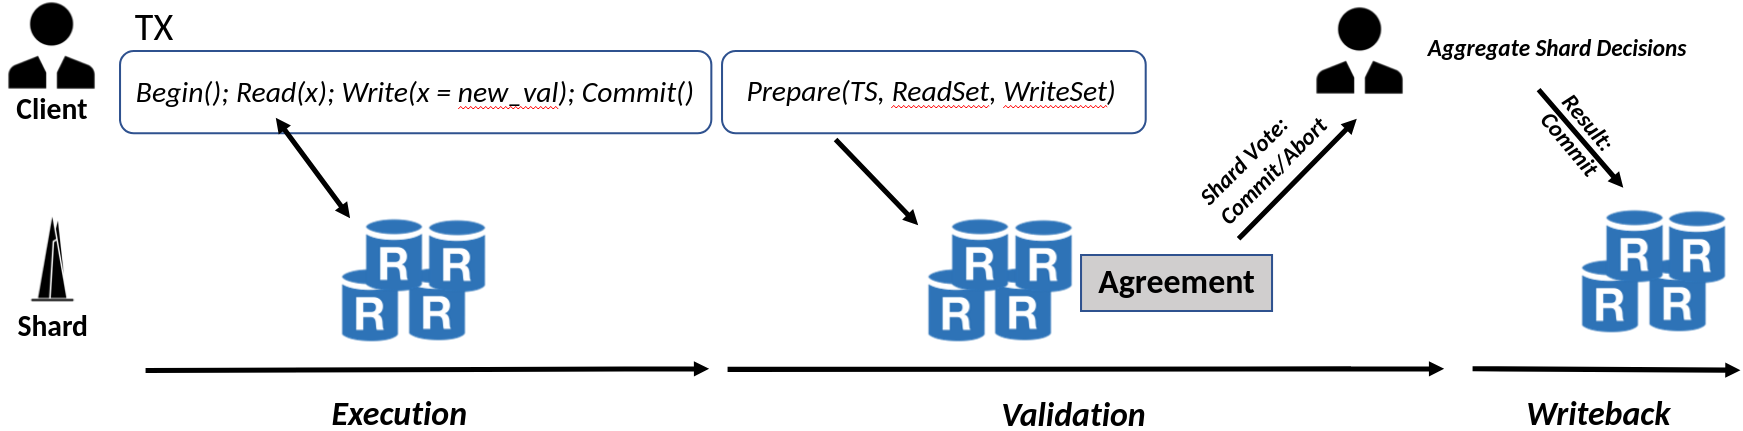
\includegraphics[width= \textwidth]{./figures/LC.png}
\end{center}
\caption{Transaction Lifecycle}
\label{fig:Figure1}
\end{figure*}
